\documentclass[11pt, fleqn]{article}
\usepackage[a4paper, hmargin={2.8cm, 2.8cm}, vmargin={2.5cm, 2.5cm}]{geometry}  % Geometri-pakke: Styrer bl.a. maginer    %
%%%%%%%%%%%%%%%%%%%%%%%%%%%%%%%%%%%%%%%%%%%%%%%%%%%%%%%%%%%%%%%%%%%%%%%%%
\usepackage[babel, stor, da]{ku-forside} % KU-forside
\usepackage[utf8]{inputenc}
\usepackage{listings}
\usepackage{amsmath}
\usepackage{amsfonts}
\usepackage{graphicx}
\usepackage[hidelinks]{hyperref}
\usepackage{pdfpages}
\usepackage{float}
\usepackage{subcaption}
\usepackage{maplestd2e}
\def\emptyline{\vspace{12pt}}
%
% Mini-manual til ku-forside pakken:
%
% Sprogmuligheder:     da, en
% babel loader babelpakken, med det valgte sprog
% Fakultetsmuligheder: farma, hum, jur, ku, life, nat, samf, sund, teo
% Farvemuligheder:     sh, farve
% Forsidemuligheder: lille, stor, titelside
%      titelside er identisk med designet på ku.dk/designmanual
%      lille er giver et lille logo sammen med titlen på den første side
%      stor er giver et stort logo sammen med titlen på den første side
%
% Default er [da,nat,farve,titelside]
%
% Ex. \usepackage[babel, lille, jur, sh, en]{ku-forside} giver et lille logo i sorthvid for juridisk fakultet og loader babelpakken med engelsk som sprog.

%%%%%%%%%%%%%%%%%%%%%%%%%%%%%%%%%%%%%%%%%%%%%%
%%%               Titel                    %%%
%%%%%%%%%%%%%%%%%%%%%%%%%%%%%%%%%%%%%%%%%%%%%%
\titel{MatIntro} %
\undertitel{Lynopgave, aflevering 9} %
%\opgave{Overspringshandling} % Findes kun under 'titelside'
\forfatter{}%
\dato{\today}%
%\vejleder{Doktoren} %  Findes kun under 'titelside'
%%%%%%%%%%%%%%%%%%%%%%%%%%%%%%%%%%%%%%%%%%%%%%%%%%%%%%%%%%%%%%%%%%
%%%                 Her begynder dokumentet                    %%%
%%%%%%%%%%%%%%%%%%%%%%%%%%%%%%%%%%%%%%%%%%%%%%%%%%%%%%%%%%%%%%%%%%
\begin{document}
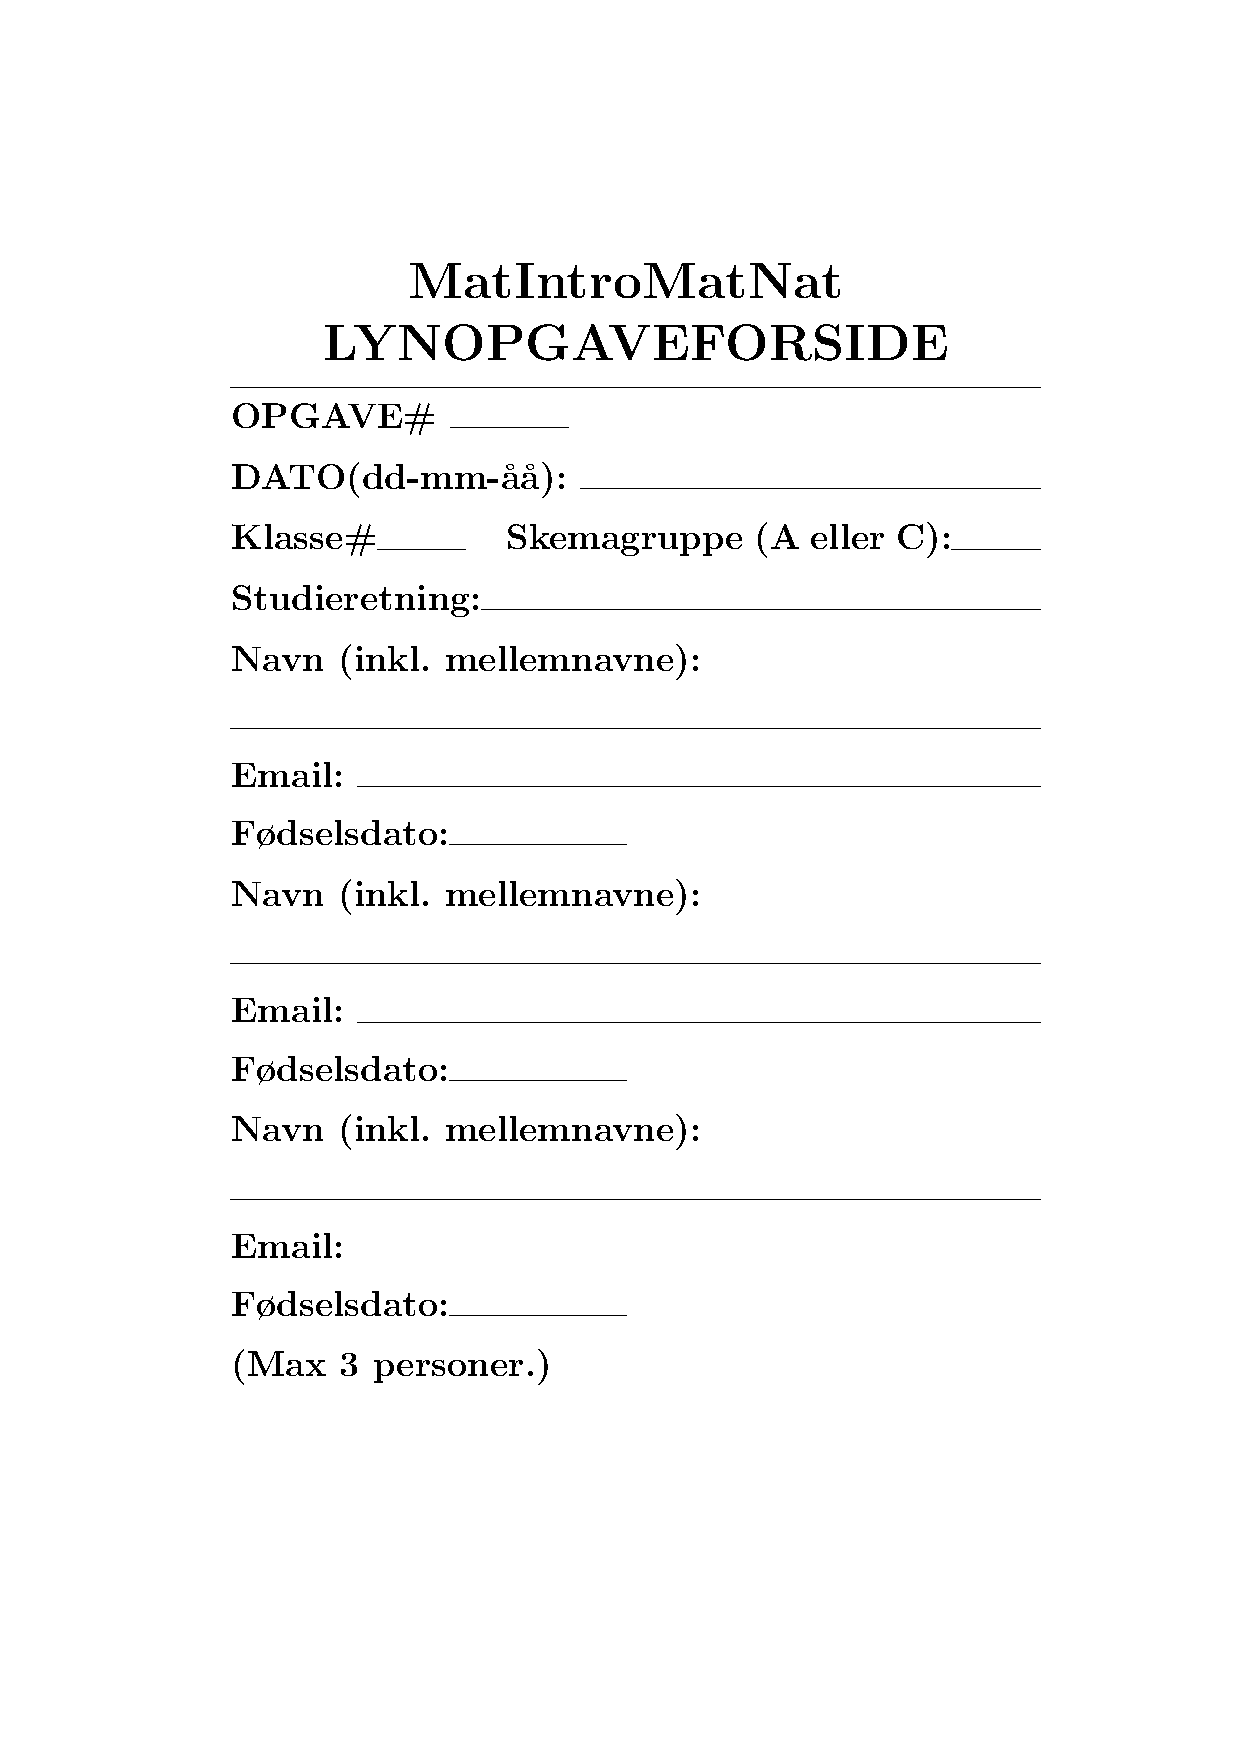
\includepdf[pages=-]{forside.pdf}
\maketitle % LAVER TITLEN
%\newpage
%%%%%%%%%%%%%%%%%%%%%%%%%%%%%%%%%%%%%%%%%%%%%%%%%%%%%%%%%%%%%%%%
%%%%%%%%%%%%%%%%%%%% TEKST BEGYNDER HER  %%%%%%%%%%%%%%%%%%%%%%%
%%%%%%%%%%%%%%%%%%%%%%%%%%%%%%%%%%%%%%%%%%%%%%%%%%%%%%%%%%%%%%%%
\section*{9.1}
\begin{equation}
\label{nostalgiccyborg}
D = \{(x,y)\ |\ 0\ \leq\ y\ \leq\ 2,\ 1-y\ \leq\ x\ \leq\ 1 \}
\end{equation}
\\
\[
	f(x,y) : D \to \mathbb{R}
\]
\begin{equation}
f(x,y) = x^2y
\end{equation}
Lad $c=0$, $d=2$, $v(y)=1-y$, $h(y)=1$. \\
Da mængden $D$ er opskrevet på formen 5.2 fra side 154 i TK, da kan planintegralet beregnes som det itererede integral opgivet ved 
\[
\int_D f(x,y) = \int^{y=2}_{y=0}\Bigg(\int^{x=1}_{x=y-1} f(x,y)\ dx \Bigg)\ dy
\]
\[
= \int^{2}_0 \bigg(\frac{1}{3}yx^3-\frac{1}{3}x^3y\bigg)\ dy = \frac{4}{5}
\]
Lad omskrivningen af mængden $D$ til formen fra 5.2 være angivet med $D'$, da skal \eqref{req1} være opfyldt. 
\begin{equation}
\label{req1}
\int_D f(x,y) = \int_{D'} f(x,y)
\end{equation}
Først kan det ses at x mindst kan være $-1$ for $y=2$, da den nedre begrænsing for $x,\ x\geq 1-y$ mindst når $y=2$. Dernæst ses det at $x$ kan være størst når $y=0,\ 1-0=1$, da er intervallet for $x,\ -1\leq x\leq 1$. \\
For at kigge på $y$ ses sammenhængen mellem $y \text{ og } x$ således fås 
\begin{align*}
1-y\leq x \\
-y \leq x-1 \\
y \geq 1-x
\end{align*}
Samtidig gælder $y$'s øvre begrænsning stadig, da fås $D'$ til 
\[
D'=\{(x,y)\ |\ -1\ \leq\ x\ \leq\ 1,\ 1-x\ \leq\ y\ \leq\ 2 \}
\]
og da er \eqref{req1} opfyldt 
\[
\int_{D} f(x,y) = 
\int_{D'} f(x,y) = 
\int_{-1}^1 \Bigg(\int_{1-x}^2\ f(x,y) dy \Bigg) dx = 
\int^{2}_{0}\Bigg(\int^{1}_{y-1} f(x,y)\ dx \Bigg)\ dy =  
\frac{4}{5}
\]

Figur \ref{badpanda} viser den figur hvis rumfang integralet $\int_D f(x,y)$ udtrykker. 
\begin{figure}[H]
\caption{Den figur hvis rumfang integralet udtrykker}
\label{badpanda}
\begin{subfigure}{.5\textwidth}
	\centering
	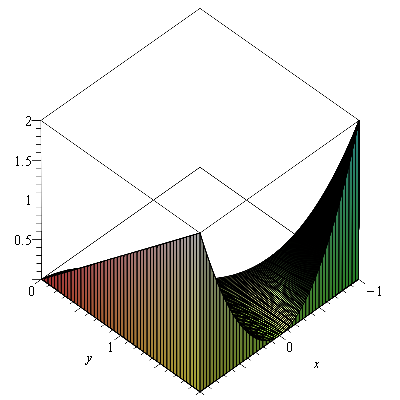
\includegraphics[scale=0.5]{grumpyskydiver}
\end{subfigure}
\begin{subfigure}{.5\textwidth}
	\centering
	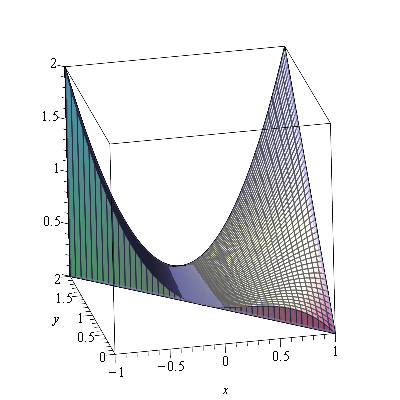
\includegraphics[scale=0.5]{sourmammal}
\end{subfigure}
\end{figure}


\end{document}